% $Id: introduction.tex 1784 2012-04-27 23:29:31Z nicolas.cardozo $
% !TEX root = main.tex

\chapter{Identification and fixing of bugs}
\label{cha:features}

We now introduce the back-in time debugger using three examples of a Management Information System (MIS) that administers grades at a university in a similar fashion as it was done to explain DeloreanJS use cases, more on the actual complete code to solve the presented problems can be found at \url{https://github.com/af-orozcog/MVI-kotlin-examples}. The following figure shows the Intellij plugin in action

\begin{figure}[h]
\centering
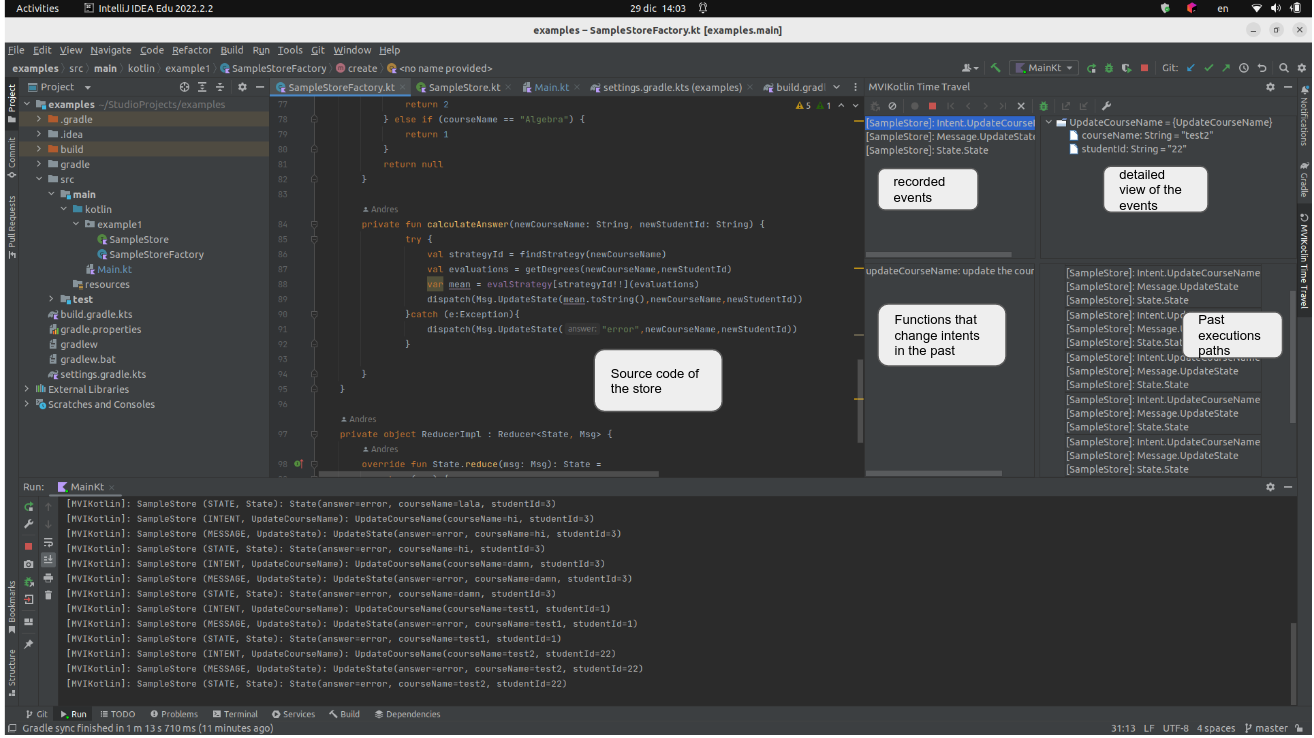
\includegraphics[height=7cm,width=13cm]{figures/Intellij}
\caption{A screenshot of the Intellij plugin}
\label{fig: A screenshot of the Intellij plugin}
\end{figure}

The plugin which is the main way to debug errors is composed of four panels, from left to right and top to bottom, the first panel shows the current events that are happening during the execution of the program. The second panel shows a detailed view of the events the user may want to examine. The third panel shows the possible functions that may be triggered to change the state of the program in a certain point on. The fourth panel shows all the previous execution paths of the program from most recent to oldest in a top to bottom fashion.

Given that most of the examples written for DeloreanJS did not have to comply with a reactive way of coding, the presented code will be an adaptation for the same problems written using reactive programming, which is based on events.

\section{Quick introduction to Stores}

In simple terms, \textbf{stores} are the objects that would enable use to go back in time. This is because they record for every moment in the program execution the state of a series of variables the developer has instructed to follow. They provide a set of "Intents" which are the events received by the \textbf{store} to update the current state. They also provide the public functions that can be called by the coder to change the state of variables in the past and re-run the program from a point on, and so enable back-in-time debugging.

\textbf{Stores} work by reacting to intents by means of an executor and a reducer. The executor would perform all the necessary operations needed to change the state (business logic), and the reducer will be the one in charge of updating it.

\textbf{Stores} are the objects that will be used through the examples to record variables, they are defined by the coder and follow the MVI architectural pattern of programming. Nonetheless, most of the examples are illustrations of the use cases and the most important pieces of implementations of the \textbf{stores} needed to represent these cases. These code pieces do not represent a complete implementation and usage of \textbf{stores}. More details on this can be found in the next chapter and in the github repository.

\section{Fix a bug}

A common task that is usually done by a system that administers grades for a university is to calculate the final grade of the course. Notice that in order to calculate the final grade different rules may apply for different courses, so it is important to know which course the grades will be calculated for. In the following example, imagine that the course was incorrectly typed and an error would always trigger, because the course name was misspelled from "Algebra" to "Alggebra", then if the programmer could simply change the name of the course to the correct one the bug would be fixed.

To be able to debug this type of event, a \textbf{store} will be created that accepts the courseName and courseId and according to that calculates the answer, which in this case is the final grade. The following is the \textbf{store} interface:

\lstset{
  columns=fullflexible,
  frame=single,
  breaklines=true,
  postbreak=\mbox{\textcolor{red}{$\hookrightarrow$}\space},
}

\begin{lstlisting}[language=java]
internal interface SampleStore: Store<Intent,State, Nothing> {
    sealed class Intent : JvmSerializable {
        data class UpdateCourseName(val courseName: String, val studentId: String) : Intent()
    }

    data class State(
        val answer: String = "",
        val courseName: String = "",
        val studentId: String = ""
    ) : JvmSerializable // Serializable only for exporting events in Time Travel, no need otherwise.
}
\end{lstlisting}

Here we can see the \textbf{store} will receive an intent specifying the courseName and studentId to trigger the calculation of the grade. This calculation part is shown in the following piece of code where we define the executor, which is the component that reacts to intents.

\begin{lstlisting}[language=java]
override fun executeIntent(intent: Intent, getState: () -> State) {
   when (intent) {
       is Intent.UpdateCourseName -> calculateAnswer(intent.courseName, intent.studentId)
   }.let {}
}

private fun calculateAnswer(newCourseName: String, newStudentId: String) {
   try {
       val strategyId = findStrategy(newCourseName)
       val evaluations = getDegrees(newCourseName,newStudentId)
       var mean = evalStrategy[strategyId!!](evaluations)
       dispatch(Msg.UpdateState(mean.toString(),newCourseName,newStudentId))
   }catch (e:Exception){
       dispatch(Msg.UpdateState("error",newCourseName,newStudentId))
   }
}

\end{lstlisting}

In the previous piece of the code given an intent to update the courseName and studentId, a function calculateAnswer is called to update the answer variable to the corresponding value either the grade of the student, or record an error in the answer. This enables us to re-run the intent with the fixed course name and re-calculate the grade of the student.

\section{Improve the Understanding of a bug}

Imagine now that the MIS system wants to get the average of the grades of a student, the grades come in the form of a matrix. This matrix could be huge for a given student, and so the time for debugging when and why an error occurs would take a significant amount of time even when using a \textbf{breakpoint}, because \textbf{breakpoints} react to the execution of a statement and are not triggered by, for example, errors. Given that MVIkotlin is based on events, we have created the following stores to simulate a for loop based on events as follows, starting with the counter interface for summing the grades of the student:

\begin{lstlisting}[language=java]
interface CounterStore: Store<Intent, State, Nothing> {
    sealed class Intent : JvmSerializable {
        data class AddValueAt(val x:Int, val y:Int, val matrix: List<List<Int>>, val state:State): Intent()
    }

    data class State(
        val counter: Int = 0,
        val state: String = ""
    ) : JvmSerializable // Serializable only for exporting events in Time Travel, no need otherwise.
}
\end{lstlisting}

Here it is seen that the counter \textbf{store} will receive an intent specifying the position of the array that the user would like to sum to the total. The next piece of code defines the executor and reducer for this \textbf{store}.

\begin{lstlisting}[language=java]
 private sealed class Msg : JvmSerializable {
        data class UpdateState(val counter: Int, val state: String) : Msg()
    }

    private inner class ExecutorImpl : CoroutineExecutor<Intent, Nothing, State, Msg, Nothing>() {
        override fun executeIntent(intent: Intent, getState: () -> State) {
            when (intent) {
                is Intent.AddValueAt -> calculateAnswer(intent.x, intent.y,intent.matrix, intent.state)
            }.let {}
        }

        private fun calculateAnswer(x: Int, y: Int, matrix: List<List<Int>>, state:State) {
            try{
                dispatch(Msg.UpdateState(matrix[x][y] + state.counter,"Successful") )
            }catch(e:Exception){
                dispatch(Msg.UpdateState(0,"Failed"))
            }
        }
    }

    private object ReducerImpl : Reducer<State, Msg> {
        override fun State.reduce(msg: Msg): State =
            when (msg) {
                is Msg.UpdateState -> copy(counter = msg.counter, state = msg.state)
            }
    }
\end{lstlisting}

The reducer and executor are very simple as they only add to the current counter the value of the entry in the matrix passed by parameter. 
In the following piece of code, is the definition of the interface of the LoopStore, this is the \textbf{store} that will be in charge of performing the operations of looping through the matrix.

\begin{lstlisting}[language=java]
interface LoopStore: Store<Intent, State, Nothing> {
    sealed class Intent : JvmSerializable {
        data class UpdateActualXAndY(val newX: Int, val newY: Int, val state:State) : Intent()
        data class UpdateN(val newN: Int,val state:State): Intent()
        data class UpdateM(val newM: Int,val state:State): Intent()
        data class UpdateXAndYAndNAndM(val newX: Int, val newY: Int, val newN: Int, val newM: Int): Intent()
        data class Start(val newN:Int, val newM:Int,val state:State) : Intent()
    }

    data class State(
        val actualX: Int = 0,
        val actualY: Int = 0,
        val N: Int = 0,
        val M: Int = 0,
        val values: List<List<Int>> = listOf(listOf(1,2),listOf(3,4))
    ) : JvmSerializable // Serializable only for exporting events in Time Travel, no need otherwise.
}
\end{lstlisting}

As it can be seen, this \textbf{store} will receive intents to start the for loop, to update the ranges of the loop and to update the current cell where it is looping. The matrix of grades of the student are also defined here which consist of a 2x2 matrix.

The following piece of code shows the executor and reducer of the loopStore.

\begin{lstlisting}[language=java]
private sealed class Msg : JvmSerializable {
   data class UpdateActualXandActualY(val newX: Int, val newY: Int) : Msg()
   data class UpdateN(val newN: Int) : Msg()
   data class UpdateM(val newM: Int) : Msg()
   data class UpdateXAndYAndNAndM(val newX: Int, val newY: Int,val newN: Int, val newM:Int) : Msg()
   data class UpdateNAndM(val newN: Int, val newM:Int) : Msg()
}

private inner class ExecutorImpl : CoroutineExecutor<Intent, Nothing, State, Msg, Nothing>() {
   override fun executeIntent(intent: Intent, getState: () -> State) {
       when (intent) {
           is Intent.UpdateN -> updateN(intent.newN, intent.state)
           is Intent.UpdateM -> updateM(intent.newM,intent.state)
           is Intent.Start -> start(intent.newN, intent.newM, intent.state)
           is Intent.UpdateXAndYAndNAndM -> updateXAndYAndNAndM(intent.newX, intent.newY, intent.newN, intent.newM)
           is Intent.UpdateActualXAndY -> updateActualXAndY(intent.newX, intent.newY, intent.state)
       }.let {}
   }

   private fun updateN(newN: Int, state: State){
       dispatch(Msg.UpdateN(newN))
       nextIteration?.let { it(state.actualX, state.actualY) }
   }

   private fun updateM(newM: Int, state: State){
       dispatch(Msg.UpdateM(newM))
       nextIteration?.let { it(state.actualX, state.actualY) }
   }

   private fun start(newN: Int, newM: Int, state: State){
       dispatch(Msg.UpdateNAndM(newN,newM))
       nextIteration?.let { it(state.actualX, state.actualY) }
   }

   private fun updateXAndYAndNAndM(newX: Int,newY: Int,newN: Int, newM: Int){
       dispatch(Msg.UpdateNAndM(newN,newM))
       nextIteration?.let { it(newX, newY) }
   }

   private fun updateActualXAndY(newX: Int, newY: Int, state: State){
       counterStore.accept(CounterStore.Intent.AddValueAt(newX,newY,state.values,counterStore.state))
       dispatch(Msg.UpdateActualXandActualY(newX,newY))
       var newNewX = newX
       var newNewY = newY + 1
       if(newNewY >= state.M){
           newNewX += 1
           newNewY = 0
       }
       if(newNewX < state.N && newNewY < state.M){
           nextIteration?.let { it(newNewX, newNewY) }
       }
   }

}

private object ReducerImpl : Reducer<State, Msg> {
   override fun State.reduce(msg: Msg): State =
       when (msg) {
           is Msg.UpdateActualXandActualY -> {
               copy(actualX = msg.newX, actualY = msg.newY)
           }

           is Msg.UpdateN -> {
               copy(N = msg.newN)
           }

           is Msg.UpdateM -> {
               copy(M = msg.newM)
           }

           is Msg.UpdateNAndM -> {
               copy(N = msg.newN, M = msg.newM)
           }
           is Msg.UpdateXAndYAndNAndM -> {
               copy(actualX = msg.newX, actualY = msg.newY, N = msg.newN, M = msg.newM)
           }
       }
}

\end{lstlisting}


Notice here that an implicit for loop is not being used to loop through the matrix, but rather a simulation of a for loop is being done by changing the entry of the array we want to sum according to the amount of rows and columns in the matrix as seen in the \textbf{updateActualXAndY} method, which sums the value in the entry \textbf{actualX} and \textbf{actualY} and then proceeds to create an intent to sum the value in the next column of the same row or next row in the first column.

Here each change of the \textbf{actualX}, \textbf{actualY}, \textbf{N} and \textbf{M} is recorded, which helps the developer check the state of the program right before an error occurred, but also change any of these parameters aiming to fix errors and check how the program would have proceeded to run from an arbitrary point on.

\section{Experiment with Hypothetical Scenarios}

In this case, the MIS system would like to calculate the average grades of a student and given this value, determine if the student got bad, good or excellent grades. Here by having a back-in-time debugger the developer would be able to experiment with the different paths of execution of the program by changing the average grades of the student. This is generally a great feature to have as exploring the different execution paths of a program without having to "re-run" the program would broaden the knowledge of the coder and help it better understand bugs in the code.

The following piece of code is the definition of the \textbf{store} interface that will tell if the student had bad, good or excellent grades.

\begin{lstlisting}[language=java]
interface HypotheticalStore: Store<Intent, State, Nothing> {
    sealed class Intent : JvmSerializable {
        data class UpdateRealMean(val realMean: Double) : Intent()
    }

    data class State(
        val answer: String = "",
        val realMean: Double? = null
    ) : JvmSerializable // Serializable only for exporting events in Time Travel, no need otherwise.
}
\end{lstlisting}

The \textbf{store} will only receive one intent with the mean of the student, and will generate the answer. The following piece of code shows the executor and reducer of the HypotheticalStore.

\begin{lstlisting}[language=java]
// Serializable only for exporting events in Time Travel, no need otherwise.
private sealed class Msg : JvmSerializable {
   data class UpdateState(val answer: String, val realMean: Double?) : Msg()
}

private inner class ExecutorImpl : CoroutineExecutor<Intent, Nothing, State, Msg, Nothing>() {
   override fun executeIntent(intent: Intent, getState: () -> State) {
       when (intent) {
           is Intent.UpdateRealMean -> calculateAnswer(intent.realMean)
       }.let {}
   }

   private fun calculateAnswer(realMean: Double) {
       try{
           if(realMean < 0.2)
               dispatch(Msg.UpdateState("bad grades",realMean))
           else if(realMean >= 0.2 && realMean < 0.8)
               dispatch(Msg.UpdateState("average grades",realMean))
           else if(realMean >= 0.8)
               dispatch(Msg.UpdateState("excellent grades",realMean))
       }catch(e:Exception){
           dispatch(Msg.UpdateState("error",null))
       }
   }
}

private object ReducerImpl : Reducer<State, Msg> {
   override fun State.reduce(msg: Msg): State =
       when (msg) {
           is Msg.UpdateState -> copy(answer = msg.answer, realMean = msg.realMean)
       }
}

\end{lstlisting}

The executor only contains a series of if statements to determine if the grades are bad, average or excellent. And the reducer updates the state.

The following is the interface of the \textbf{store} that is in charge of calculating the average of the student.

\begin{lstlisting}[language=java]
interface HelperStore: Store<Intent, State, Nothing>  {
    sealed class Intent : JvmSerializable {
        data class UpdateRealMean(val realMean: Double) : Intent()
        data class UpdateStudentId(val studentId: String): Intent()
    }

    data class State(
        val studentId: String = "",
        val realMean: Double? = null,
        val state: String = ""
    ) : JvmSerializable // Serializable only for exporting events in Time Travel, no need otherwise.
}
\end{lstlisting}

This \textbf{store} receives intents to either update the mean of the grades of the student or update the student the developer would like to calculate the mean of the grades for.

The following fragment of code shows the executor and reducer for this HelperStore.

\begin{lstlisting}[language=java]
// Serializable only for exporting events in Time Travel, no need otherwise.
private sealed class Msg : JvmSerializable {
   data class UpdateState(val studentId: String, val realMean:Double?, val state:String) : Msg()
   data class UpdateRealMean(val realMean:Double): Msg()
}

private inner class ExecutorImpl : CoroutineExecutor<Intent, Nothing, State, Msg, Nothing>() {
   override fun executeIntent(intent: Intent, getState: () -> State) {
       when (intent) {
           is Intent.UpdateStudentId -> calculateAnswer(intent.studentId)
           is Intent.UpdateRealMean -> updateRealMean(intent.realMean)
       }.let {}
   }

   private fun updateRealMean(realMean: Double){
       dispatch(Msg.UpdateRealMean(realMean))
       hypotheticalStore.accept(HypotheticalStore.Intent.UpdateRealMean(realMean))
   }

   private fun calculateAnswer(studentId: String) {
       try{
           if(studentId == "1") {
               dispatch(Msg.UpdateState(studentId, 0.8, "Succesful"))
               hypotheticalStore.accept(HypotheticalStore.Intent.UpdateRealMean(0.8))
           }
           else if(studentId == "2") {
               dispatch(Msg.UpdateState(studentId, 0.1, "Succesful"))
               hypotheticalStore.accept(HypotheticalStore.Intent.UpdateRealMean(0.1))
           }
           else if(studentId == "3") {
               dispatch(Msg.UpdateState(studentId, 0.3, "Succesful"))
               hypotheticalStore.accept(HypotheticalStore.Intent.UpdateRealMean(0.3))
           }
           else if(studentId == "4") {
               dispatch(Msg.UpdateState(studentId, 0.5, "Succesful"))
               hypotheticalStore.accept(HypotheticalStore.Intent.UpdateRealMean(0.5))
           }
       }catch(e:Exception){
           dispatch(Msg.UpdateState("", null, "Failed"))
       }
   }
}

private object ReducerImpl : Reducer<State, Msg> {
   override fun State.reduce(msg: Msg): State =
       when (msg) {
           is Msg.UpdateState -> copy(studentId = msg.studentId, realMean = msg.realMean, state = msg.state)
           is Msg.UpdateRealMean -> copy(realMean = msg.realMean)
       }
}
\end{lstlisting}

Here the executor would either receive messages to change the studentId or the mean of the grades of the current student defined in the state. This always triggers an update in the evaluation of the grades of the student in the HypotheticalStore, possibly triggering a different execution path.

\endinput

